\section{Performance \& problems}
\label{sec:performance}
The project was developed and tested on an Intel Core i5-10600 clocked at 3.3~GHz with 16~GB of RAM and NVIDIA RTX 2060 SUPER. The simulations were tested in the 500,000 data samples and 60,000 render samples configuration to achieve maximum resolution. There are significant differences in the performance of Driftworld Tectonics and the procedural method by Cortial et al. The 500,000 data sample does not allow for smooth interactivity, possibly due to the dependence on internal Unity mechanisms and limited optimization. A~single tectonic step takes between 3-10 seconds, depending on continental collisions and rifting events. Arguably, a~credible landmass layout can be achieved in around 60 steps when using laplacian smoothing and/or manual elevation. Datawise, the output is robust enough to not cause serious incorrigible artifacts. An example of a fully formed continent after 59 steps using standard configuration (see summaries of the model and implementation, tables \ref{tab:model-parameters-summary} and \ref{tab:implementation-parameters-summary}) is seen in Figure~\ref{fig:output-example}.
\begin{figure}[ht]
\centering
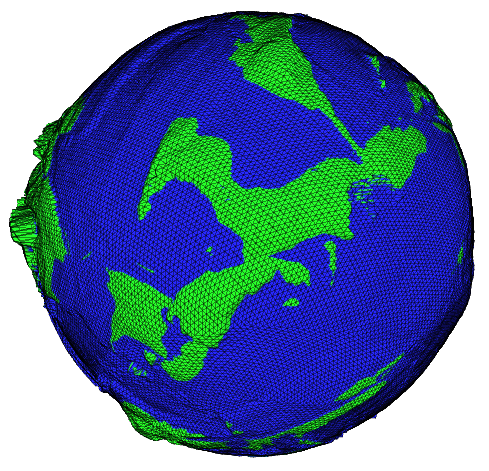
\includegraphics[height=13cm]{performance-continent.png}
\caption{Continental ladmass - example of the simulation output}
\label{fig:output-example}
\end{figure}

Configurations with 60,000 data samples or less are much faster, although they do suffer from decreased resolution, especially around crust borders. This, however, should be mitigated by proper terrain amplification.

The initial number of tectonic plates has a~performance consequences for the simulations. Higher number of plates implies larger subduction fronts and thus more landmass is created, while lower number of plates causes landmass to actually decrease in size. It is therefore convenient to keep the number of plates as high as possible.

Driftworld Tectonics performance has several issues that can possibly be addressed by further optimalization. Following subsections describe the most prominent issues and how to counter them.

\subsection{Interpolation artifacts}
Layer data is interpolated many times during a simulation and on certain conditions the results are imprecise. This is mostly prominent on perfectly flat surfaces and along crust plate borders. The artifacts show as peaks on the surface and have most frequently the size of a single sample point. These very quickly disappear when actual tectonic steps are performed, as the terrain is no longer flat and any artifacts are hidden within the complexity of the terrain (see Figure \ref{fig:issue-interpolation}).
\begin{figure}[ht!]
\centering
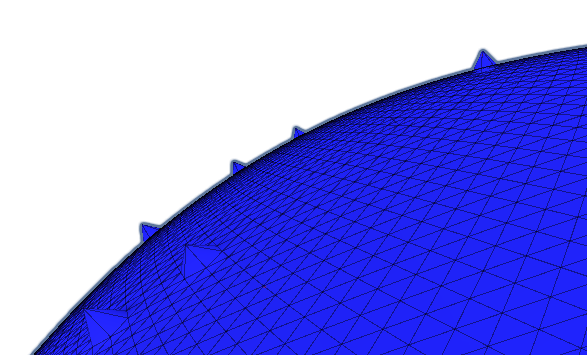
\includegraphics[height=9cm]{issue-interpolation.png}
\caption{Flat surface peaks - interpolation imperfections}
\label{fig:issue-interpolation}
\end{figure}

\subsection{Missing texture data}
Calculations of overlay textures relies heavily on interpolation. Any falsely negative triangle tests because of precision errors result in 'dead' pixels in the texture. This is purely a rendering issue and does not pose a problem for the simulation (see Figure \ref{fig:issue-dead-pixels}).
\begin{figure}[ht!]
\centering
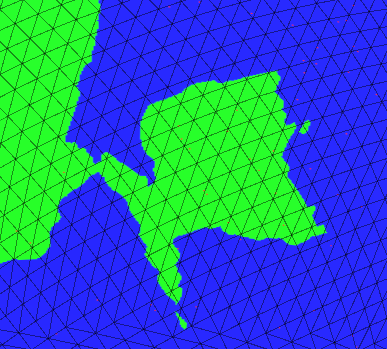
\includegraphics[height=9cm]{performance-B.png}
\caption{Missing texture data}
\label{fig:issue-dead-pixels}
\end{figure}

\subsection{Smoothing borders}
As a direct result of a terrain smoothing, borders are somewhat simplified, which may cause an unnatural look, especially when it is overused. This can be improved by adding tectonic steps without smoothing but sometimes it is better to load a previous state of the simulation and look for another way (see Figure \ref{fig:issue-blobs}).
\begin{figure}[ht!]
\centering
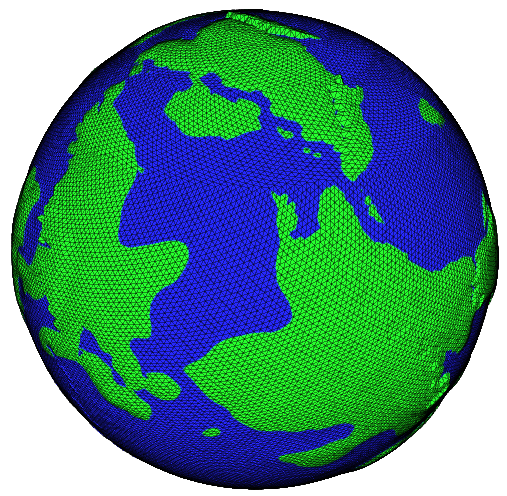
\includegraphics[height=9cm]{performance-A.png}
\caption{Unnatural smoothing of continental shores}
\label{fig:issue-blobs}
\end{figure}

\begin{figure}[ht!]
\centering
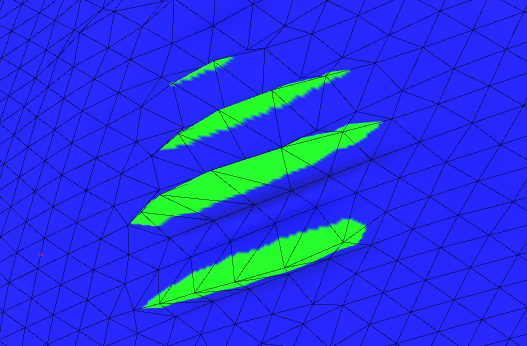
\includegraphics[height=9cm]{issue-furrows.png}
\caption{Crust furrows}
\label{fig:crust-furrows}
\end{figure}

\subsection{Compute shader crashes}
For high sample count simulations (500,000 data samples), computations on the crust layer stretch GPU compute shaders to their limits. For crust plates number exceeding 30, tectonic steps sometimes cause crashes on compute shader dispatches. This is the main reason why the recommended initial number of plates is 20. For lower number of samples, 40 plates is a~viable option and should be used to create more interesting crust formations. The lower number of plates can be counter-weighted by applying manual elevation increments, such as in the example in Figure  \ref{fig:output-example}. It is possible that a~better GPU might not have the same issues, but this was not tested.
\subsection{Memory leaks}
The simulations of 500,000 data samples are somewhat RAM-intensive. After many tectonic and rendering steps, the simulation may continuously increase its used operational memory. This is obviously due to memory leaks, which may have two probable causes: constant resampling of the crust or memory lost due to texture reassignments. Until the problem is properly addressed, it is recommended that users periodically save their simulations to files and then load them to restarted Unity editor scenes. The rate of the memory increase is small but steady -- 100 tectonic steps with renders seem to increase the required memory by about 5 GB at 500,000 data samples.
\subsection{Past issues}
During a simulation after 20-30 steps, crust artifacts used to occur where the terrain was creased along one direction (see Figure \ref{fig:crust-furrows}). These artifacts were caused by incorrectly normalized barycentric interpolation and subsequent crust resampling. This normalization has since been improved.
